\documentclass{article}

\usepackage{fancyhdr}
\usepackage{extramarks}
\usepackage{amsmath}
\usepackage{amsthm}
\usepackage{amsfonts}
\usepackage{tikz}
\usepackage[plain]{algorithm}
\usepackage{algpseudocode}
\usepackage{graphicx}
\usetikzlibrary{automata,positioning}
\usepackage{pdfpages,float}

%
% Basic Document Settings
%

\topmargin=-0.45in
\evensidemargin=0in
\oddsidemargin=0in
\textwidth=6.5in
\textheight=9.0in
\headsep=0.25in

\linespread{1.1}

\pagestyle{fancy}
\lhead{\hmwkAuthorName}
\chead{\hmwkClass\ (\hmwkClassInstructor\ \hmwkClassTime): \hmwkTitle}
\rhead{\firstxmark}
\lfoot{\lastxmark}
\cfoot{\thepage}

\renewcommand\headrulewidth{0.4pt}
\renewcommand\footrulewidth{0.4pt}

\setlength\parindent{0pt}

%
% Create Problem Sections
%

\newcommand{\enterProblemHeader}[1]{
    \nobreak\extramarks{}{Problem \arabic{#1} continued on next page\ldots}\nobreak{}
    \nobreak\extramarks{Problem \arabic{#1} (continued)}{Problem \arabic{#1} continued on next page\ldots}\nobreak{}
}

\newcommand{\exitProblemHeader}[1]{
    \nobreak\extramarks{Problem \arabic{#1} (continued)}{Problem \arabic{#1} continued on next page\ldots}\nobreak{}
    \stepcounter{#1}
    \nobreak\extramarks{Problem \arabic{#1}}{}\nobreak{}
}

\setcounter{secnumdepth}{0}
\newcounter{partCounter}
\newcounter{homeworkProblemCounter}
\setcounter{homeworkProblemCounter}{1}
\nobreak\extramarks{Problem \arabic{homeworkProblemCounter}}{}\nobreak{}

%
% Homework Problem Environment
%
% This environment takes an optional argument. When given, it will adjust the
% problem counter. This is useful for when the problems given for your
% assignment aren't sequential. See the last 3 problems of this template for an
% example.
%
\newenvironment{homeworkProblem}[1][-1]{
    \ifnum#1>0
        \setcounter{homeworkProblemCounter}{#1}
    \fi
    \section{Problem \arabic{homeworkProblemCounter}}
    \setcounter{partCounter}{1}
    \enterProblemHeader{homeworkProblemCounter}
}{
    \exitProblemHeader{homeworkProblemCounter}
}

%
% Homework Details
%   - Title
%   - Due date
%   - Class
%   - Section/Time
%   - Instructor
%   - Author
%

\newcommand{\hmwkTitle}{Homework\ \#9}
\newcommand{\hmwkDueDate}{Nov 17, 2019}
\newcommand{\hmwkClass}{CMSE 820}
\newcommand{\hmwkClassTime}{}
\newcommand{\hmwkClassInstructor}{Professor Yuying Xie}
\newcommand{\hmwkAuthorName}{\textbf{Boyao Zhu}}

%
% Title Page
%

\title{
    \vspace{2in}
    \textmd{\textbf{\hmwkClass:\ \hmwkTitle}}\\
    \normalsize\vspace{0.1in}\small{Due\ on\ \hmwkDueDate\ at 11:59pm}\\
    \vspace{0.1in}\large{\textit{\hmwkClassInstructor\ \hmwkClassTime}}
    \vspace{3in}
}

\author{\hmwkAuthorName}
\date{}

\renewcommand{\part}[1]{\textbf{\large Part \Alph{partCounter}}\stepcounter{partCounter}\\}

%
% Various Helper Commands
%

% Useful for algorithms
\newcommand{\alg}[1]{\textsc{\bfseries \footnotesize #1}}

% For derivatives
\newcommand{\deriv}[1]{\frac{\mathrm{d}}{\mathrm{d}x} (#1)}

% For partial derivatives
\newcommand{\pderiv}[2]{\frac{\partial}{\partial #1} (#2)}

% Integral dx
\newcommand{\dx}{\mathrm{d}x}

% Alias for the Solution section header
\newcommand{\solution}{\textbf{\large Solution}}

% Probability commands: Expectation, Variance, Covariance, Bias
\newcommand{\E}{\mathrm{E}}
\newcommand{\Var}{\mathrm{Var}}
\newcommand{\Cov}{\mathrm{Cov}}
\newcommand{\Bias}{\mathrm{Bias}}

\begin{document}

\maketitle

\pagebreak

\begin{homeworkProblem}

\textbf{Solution}\\
(a) Figure 1
(b) After makeing the change in the dataset, the dataset becomes non-separable linearly, so hard margin SVM yields no solution.
(c) Figure 2
\begin{figure}
	\centerline{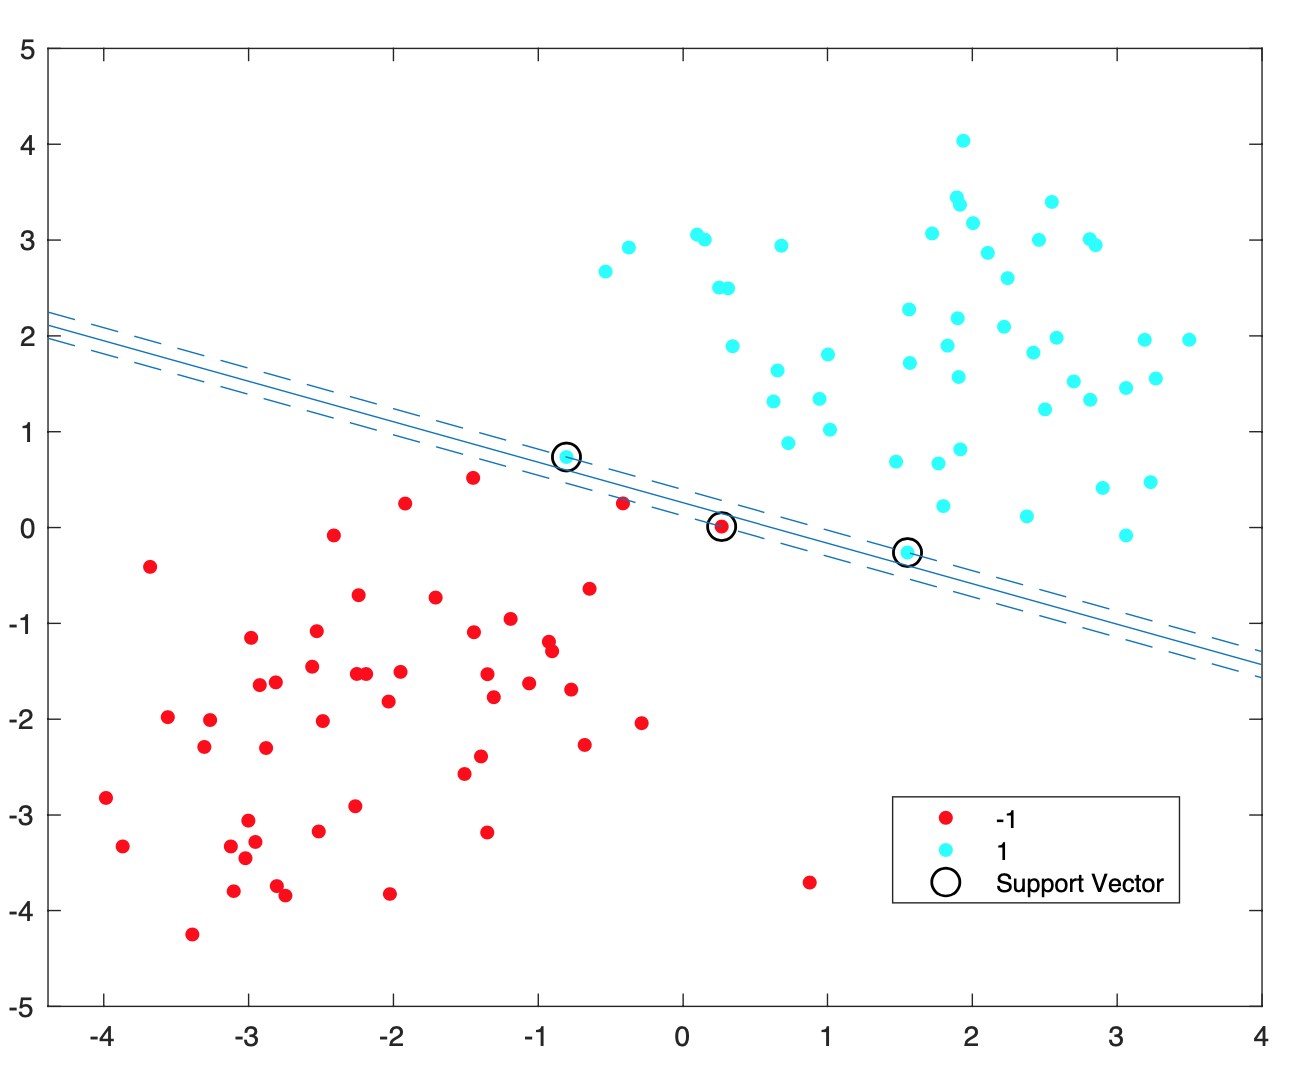
\includegraphics[scale=0.3]{HW9a.png}}
	\caption{Hard margin SVM on a separable dataset.  The colors indicate the original label in the data set}
\end{figure}



\begin{figure}[H]
	\centerline{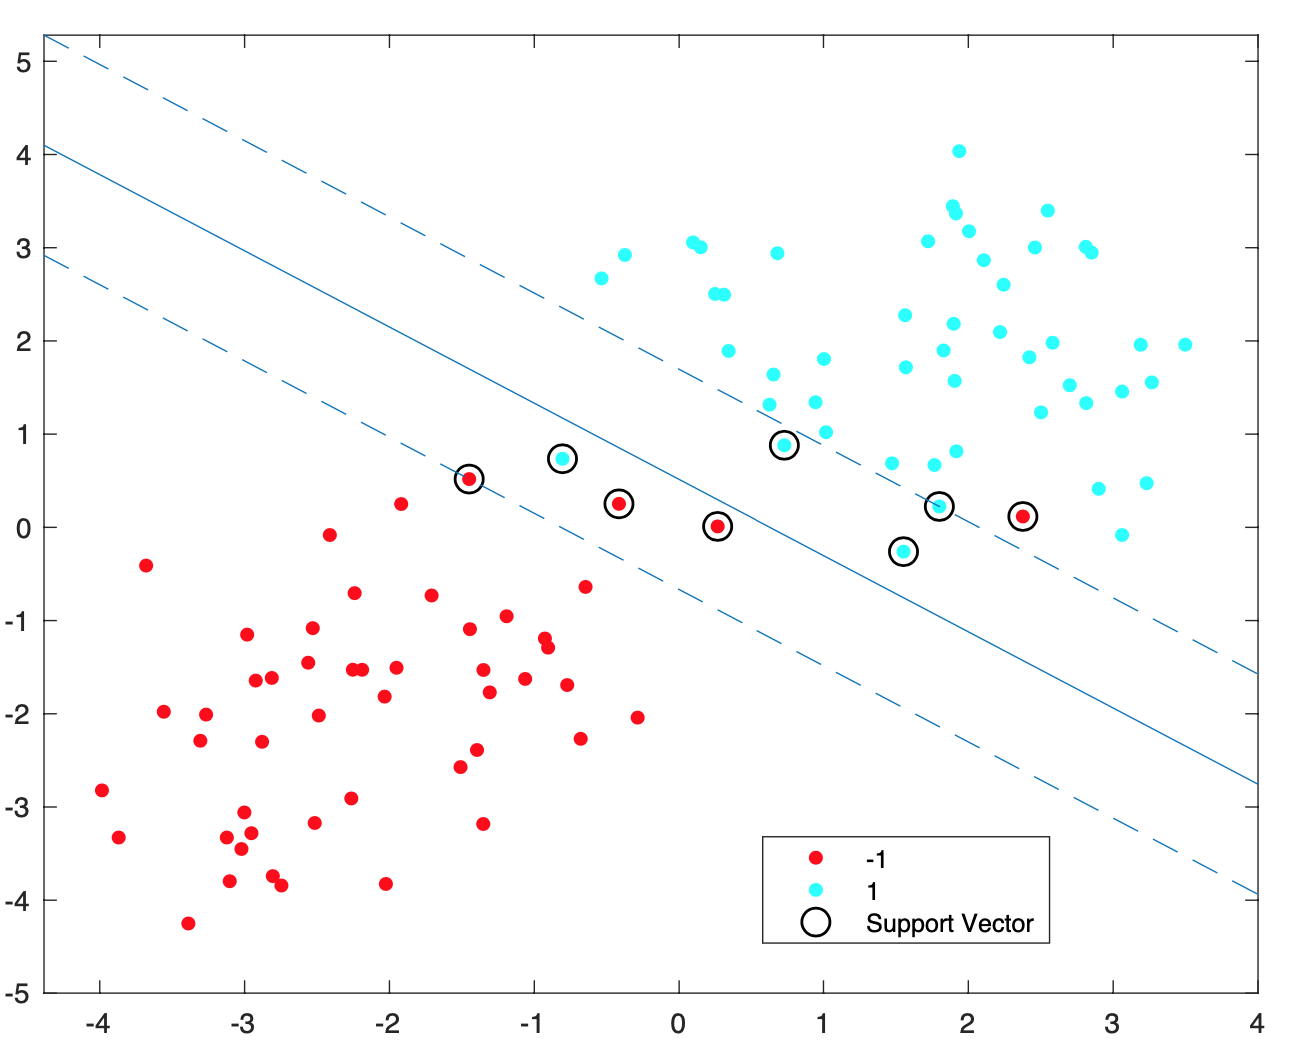
\includegraphics[scale=0.3]{HW9_2.png}}
	\caption{Soft margin SVM on a non-separable dataset.  The colors indicate the original label in the dataset.}
\end{figure}


\end{homeworkProblem}





\begin{homeworkProblem}
\textbf{Solution}\\
Figure 3\\

Figure 4\\
Figure 5\\
\begin{figure}
	\centerline{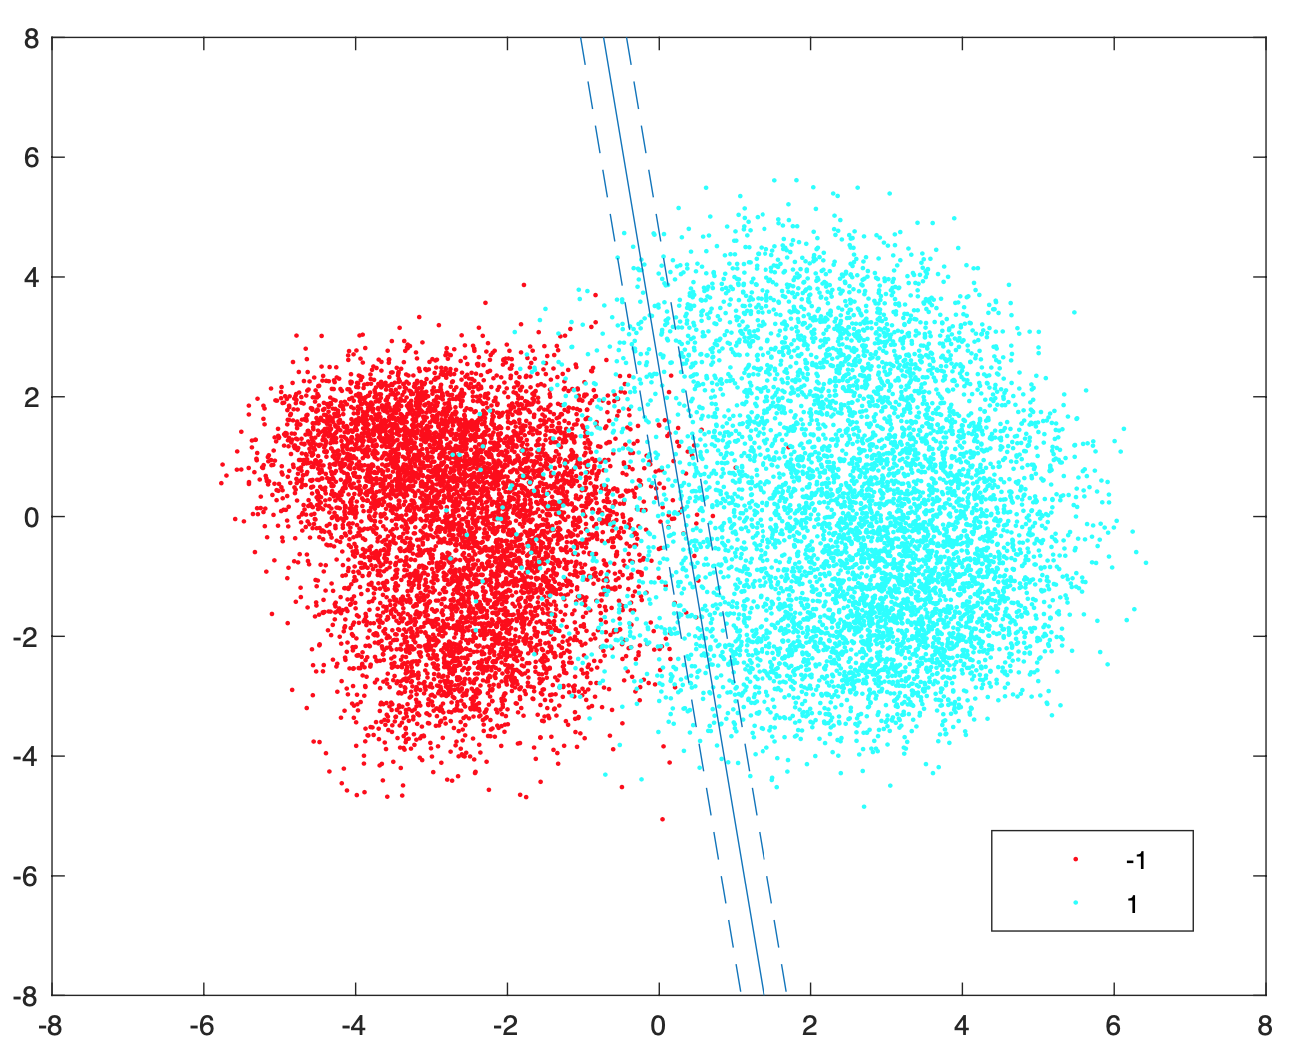
\includegraphics[scale=0.3]{3.png}}
	\caption{Hard margin SVM on the original dataset.  The solid line is the intersection of the SVM hyperplane and the plane spanned by the top 2 PCs.}
\end{figure}


\begin{figure}
	\centerline{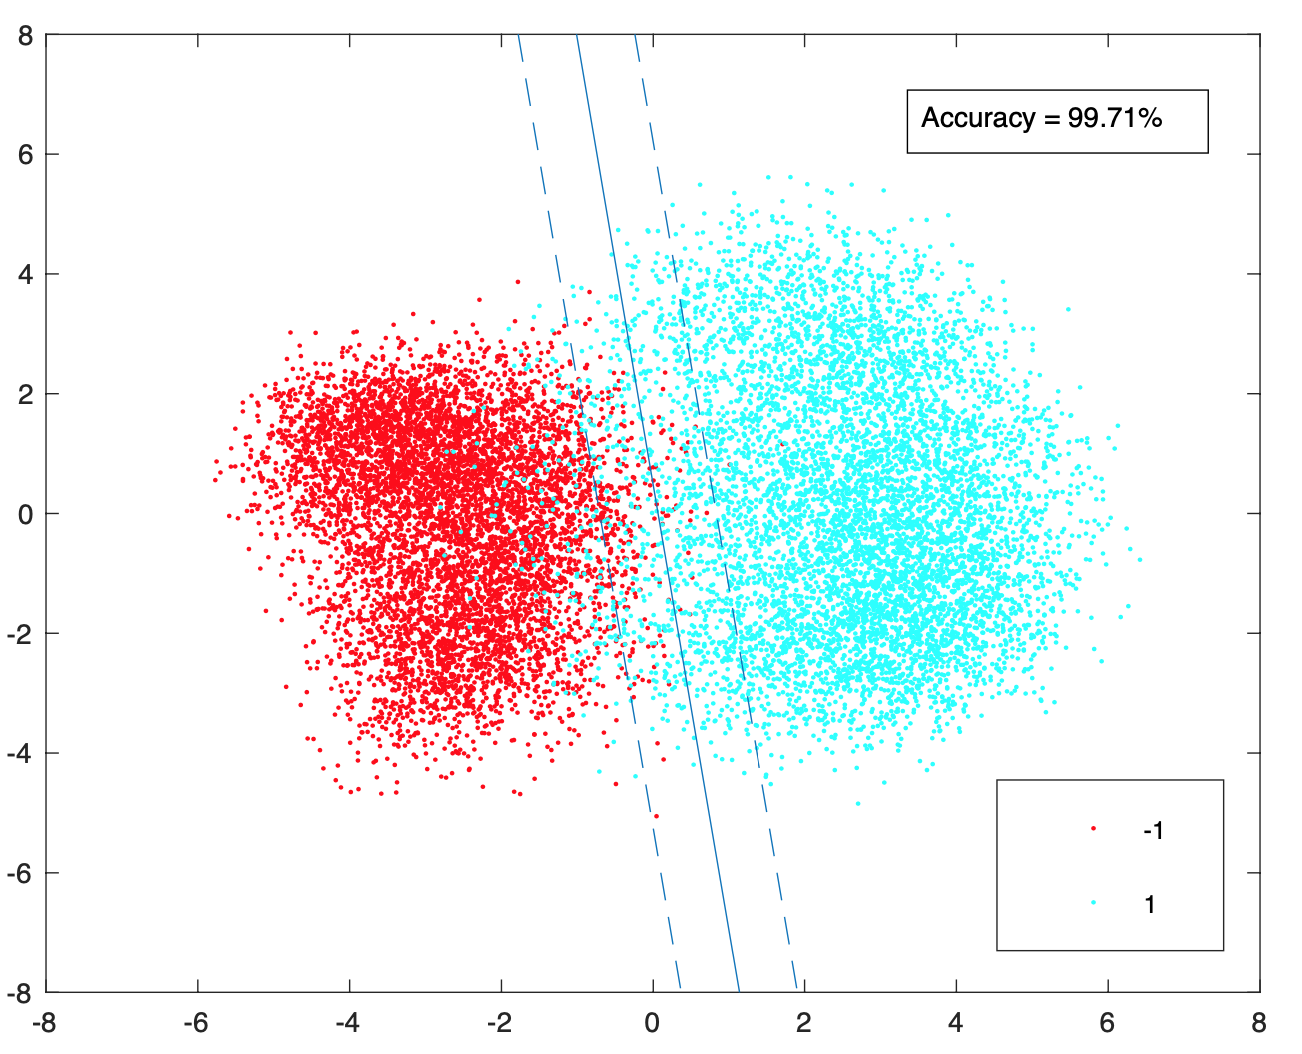
\includegraphics[scale=0.3]{4.png}}
	\caption{Soft margin SVM on the original dataset.  The solid line is the intersection of the SVM hyperplane and the plane spanned by the top 2 PCs.}
\end{figure}



\begin{figure}
	\centerline{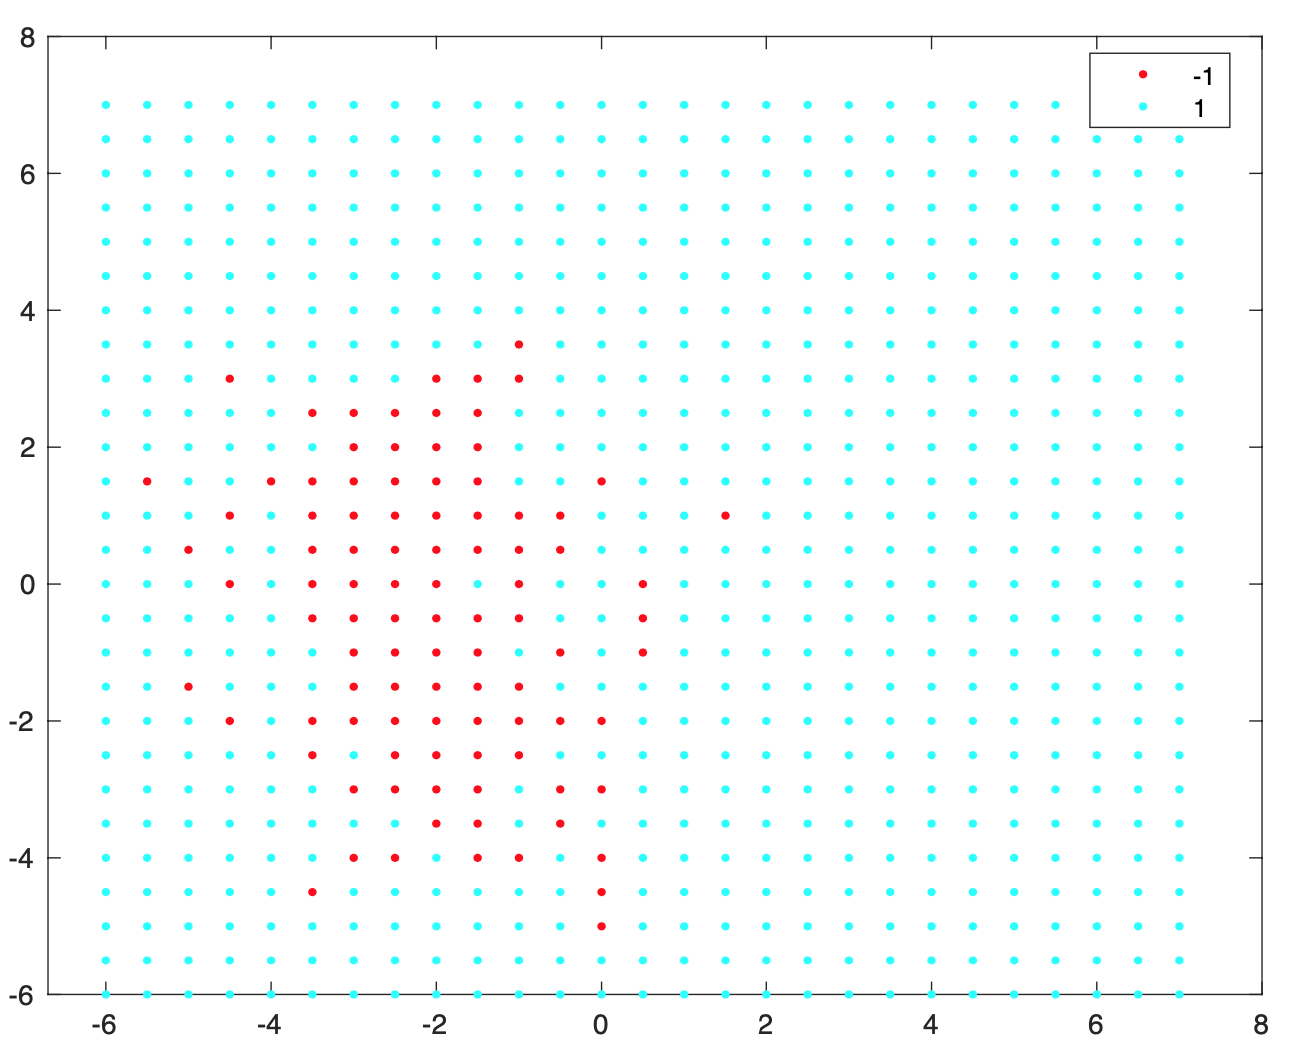
\includegraphics[scale=0.3]{5.png}}
	\caption{Predictions of the SVM model with a Gaussian kernel on the grid spanned along the top 2 PCs.}

\end{figure}

\end{homeworkProblem}






\begin{homeworkProblem}
Soft Margin SVM\\
(1) Regularized risk form:
\[
\underset{w,b}{\text{min}}\sum_i[1-y_i(\langle w,x_i\rangle+b)]_+ +\frac{\lambda}{2}\lVert w\rVert^2
\]
(2) Primal form:
\[
\begin{split}
&\underset{w,b}{\text{min}}\gamma\sum_i\xi_i+\frac{1}{2}\lVert w\rVert^2\\
&\text{subject to } \xi_i>0, \quad y_i(\langle w,x_i\rangle+b) \geq 1-\xi_i
\end{split}
\]
Show that they are equivalent with \(\lambda=\frac{1}{\gamma}\).\\
\\
\textbf{Solution}\\ 
Substituting \(\lambda = \frac{1}{\lambda}\), the regularized risk form problem can be rewritten as 
\[
\underset{w,b}{\text{min}}\gamma\sum_i\text{max}\{0, 1-y_i(\langle w,x_i\rangle+b)\}+\frac{1}{2}\lVert w\rVert^2
\]
Let \(\{w_1,b_1\} \text{ and } \{w_2,b_2\}\) denote respectively the optimal solutions to the regularized risk form problem and the primal problem respectively.\\
The Lagrangian for the primal problem reads
\[
L(w,b,\xi_i,\alpha_i,\lambda_i) = \gamma\sum_i\xi_i+\frac{1}{2}\lVert w\rVert^2 + \sum_i\alpha_i[1-\xi_i-y_i(\langle w,x_i\rangle+b)]-\sum_i\lambda_i\xi_i
\]
The complementary slackness yields
\[
\forall i, \lambda_i\xi_i = 0 \text{ and } \alpha_i[1-\xi_i-y_i(\langle w_2,x_i\rangle+b_2)] = 0
\]
So the objective function of the primal problem at the optimal solution \(\{w_2,b_2\}\) is given by
\[
\gamma\sum_i\text{max}\{0,1-y_i(\langle w_2,x_i\rangle+b_2)\} + \frac{1}{2}\lVert w_2\rVert^2 \geq \gamma\sum_i\text{max}\{0,1-y_i(\langle w_1,x_i\rangle+b_1)\} + \frac{1}{2}\lVert w_1\rVert^2
\]
The inequality follows from that \(\{w_1,b_1\}\) is the optimal solution to the regularized form problem.\\
On the other hand, given \(\{w_1,b_1\}\), we can define \(\xi_i' := \text{max}\{0, 1-y_i(\langle w_1,x_i\rangle+b_1)\}\) such that \(\xi_i'\) is feasible for the primal form problem.  The optimality of the primal form solution \(\{w_2,b_2\}\) gives
\[
\gamma\sum_i\text{max}\{0, 1-y_i(\langle w_2,x_i\rangle+b_2)\} + \frac{1}{2}\lVert w_2\rVert^2 \leq \gamma\sum_i\text{max}\{0,1-y_i(\langle w_1,x_i\rangle+b_1)\} + \frac{1}{2}\lVert w_1\rVert^2
\]
We obtain an equality from the previous two inequalities
\[
\gamma\sum_i\text{max}\{0, 1-y_i(\langle w_2,x_i\rangle+b_2)\} + \frac{1}{2}\lVert w_2\rVert^2 = \gamma\sum_i\text{max}\{0,1-y_i(\langle w_1,x_i\rangle+b_1)\} + \frac{1}{2}\lVert w_1\rVert^2
\]
Moreover, since the soft margin SVM problem is a strictly convex optimization problem, the solution is unique, i.e.,
\[
w_1 = w_2 \text{ and } b_1 = b_2.
\]
Thus, the two forms of problems are equivalent.

\end{homeworkProblem}



\begin{homeworkProblem}
Constrained form:
\[
\underset{x}{\text{min}}f(x) \quad \text{subject to}\quad h(x)\leq t
\]
Lagrange form:
\[
\underset{x}{\text{min}}f(x) +\lambda h(x)
\]
Show that they are Equivalent?\\
\\
\textbf{Solution}\\
First of all, they are not equivalent in general.  A counterexample: If we let \(f(x) = x, h(x) = -x \text{ and } t =1\), then there exists no \(\lambda\) that can help the Lagrange form to yield the same solution.\\
\\
\textbf{Given a} \(t\), \textbf{what should} \(\lambda\) \textbf{be such that the Lagrange form yields the same solution as the constrained form?}\\
\\
We have to impose a few extra conditions: (1) both \(f(x)\) and \(h(x)\) are at least twice differentiable; (2) the function \(g(x) := -f'(x)/h'(x)\) is well-defined and strictly monotonic; (3) the function \(j(x) = f''(x) + g(x)h''(x)\) is well-defined and strictly positive.\\
For any given \(t\), let's denote the optimal solution to the constrained problem as \(\tilde{x}(t)\).  We claim that when
\[
\lambda(t) = -f'[\tilde{x}(t)]/h'[\tilde{x}(t)]
\]
the Lagrange form problem is equivalent to the constrained form problem.  Taking the derivative of the Lagrangian \(L(x) = f(x) - \frac{f'[\tilde{x}(t)]}{h'[\tilde{x}(t)]}h(x)\) and setting it to 0 gives,
\[
f'(x)-\frac{f'[\tilde{x}(t)]}{h'[\tilde{x}(t)]}h'(x)=0
\]
Since the function \(-f'(x)/h'(x)\) is strictly monotonic, the only possible solution is given by \(x=\tilde{x}(t)\).  Indeed, \(x=\tilde{x}(t)\) is the optimal solution to the Lagrange problem because \(L''(\tilde{x}(t))>0\) by assumption (3).\\
\\
\textbf{Given a }\(\lambda>0\), \textbf{what should } \(t\) \textbf{be such that the constrained form yields the same solution as the Lagrange form?}\\
\\
Let's denote \(x^\ast(\lambda)\) as the optimal solution to the Lagrange problem and \(\tilde{x}(t)\) as the optimal solution to the constrained problem.  We claim that
\[
t(\lambda) = h[x^\ast(\lambda)]
\]
The optimality of \(x^\ast(\lambda)\) for the Lagrange problem implies that
\[
\forall x\in\{x : h(x)\leq h[x^\ast(\lambda)]\}, f[x^\ast(\lambda)] + \lambda h[x^\ast(\lambda)]\leq f(x) + \lambda h(x) \leq f(x)+\lambda h[x^\ast(\lambda)]
\]
which implies that \(f[x^\ast(\lambda)]\leq f(x)\) for all feasible \(x\) in the constrained problem.  So \(x^\ast(\lambda)\) is a solution to the constrained problem as well.
\end{homeworkProblem}


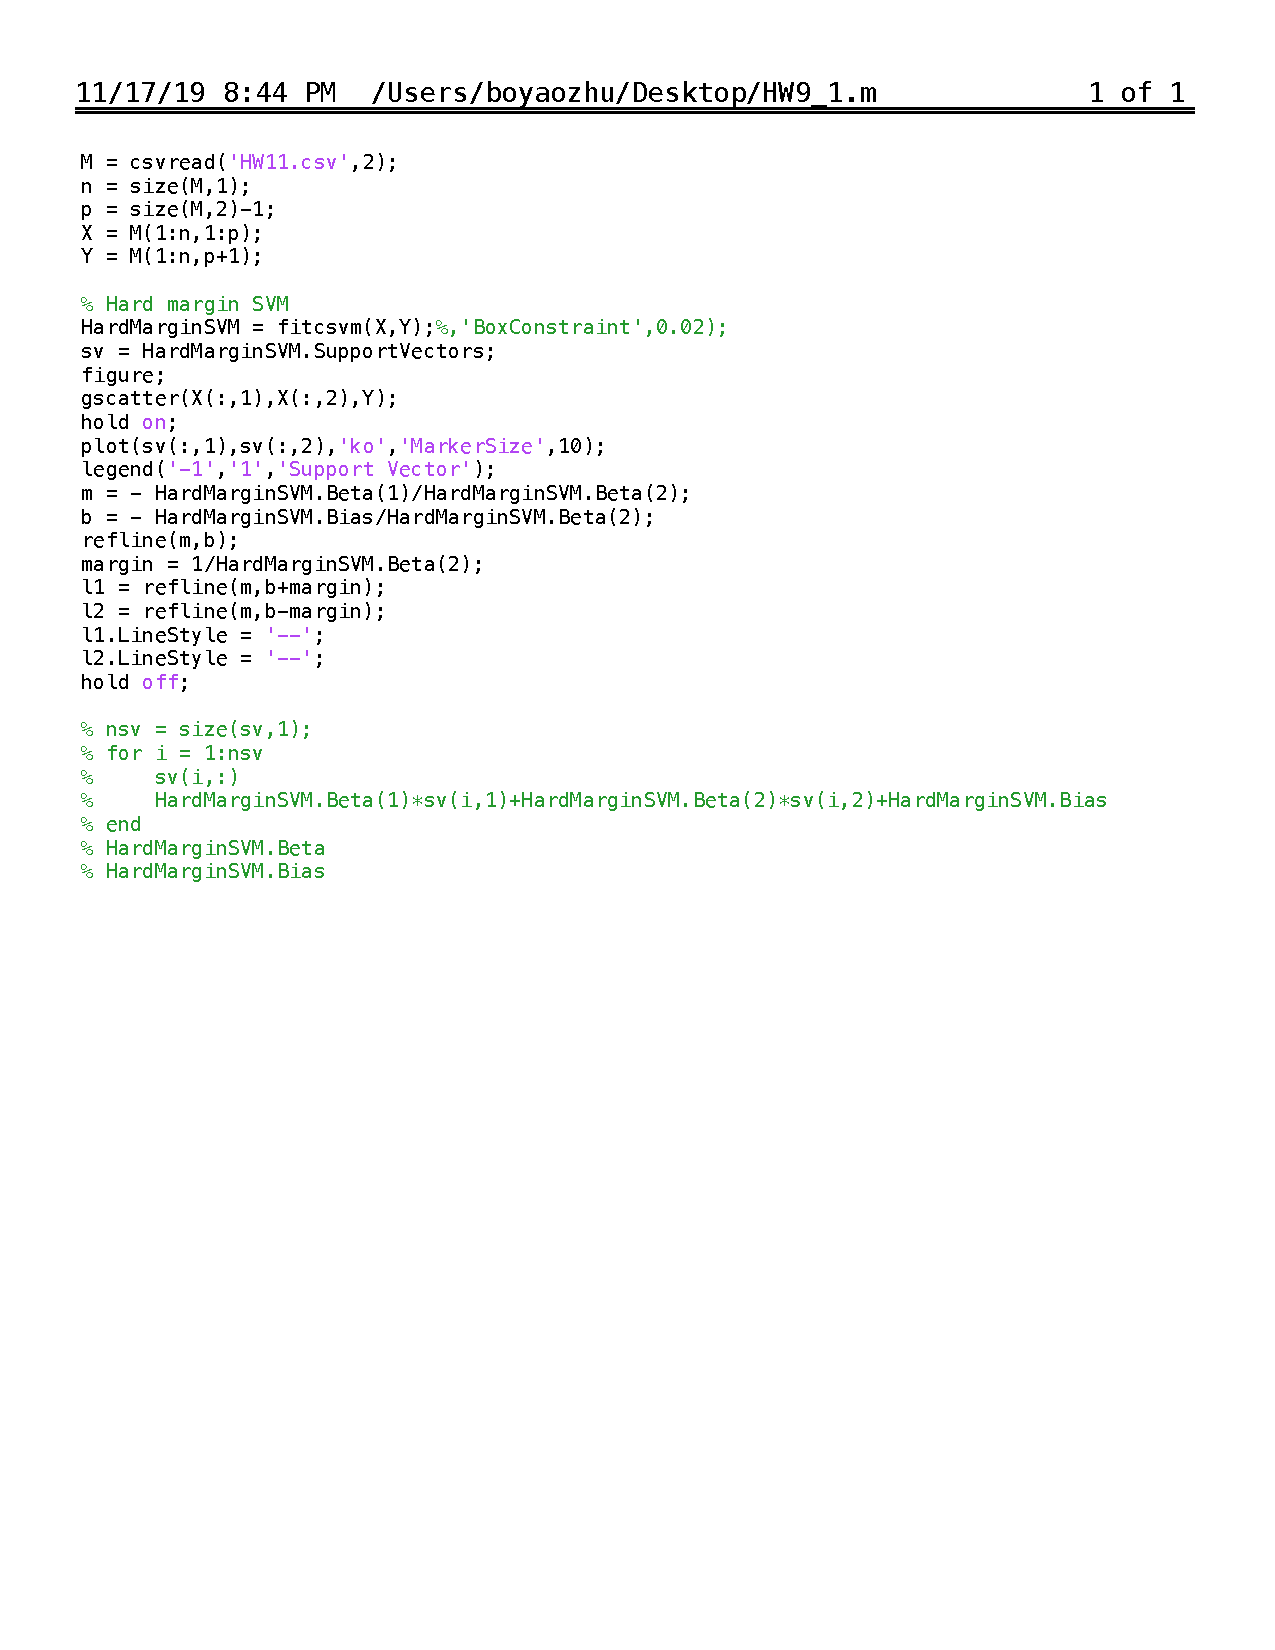
\includepdf[page={-}]{1.pdf}
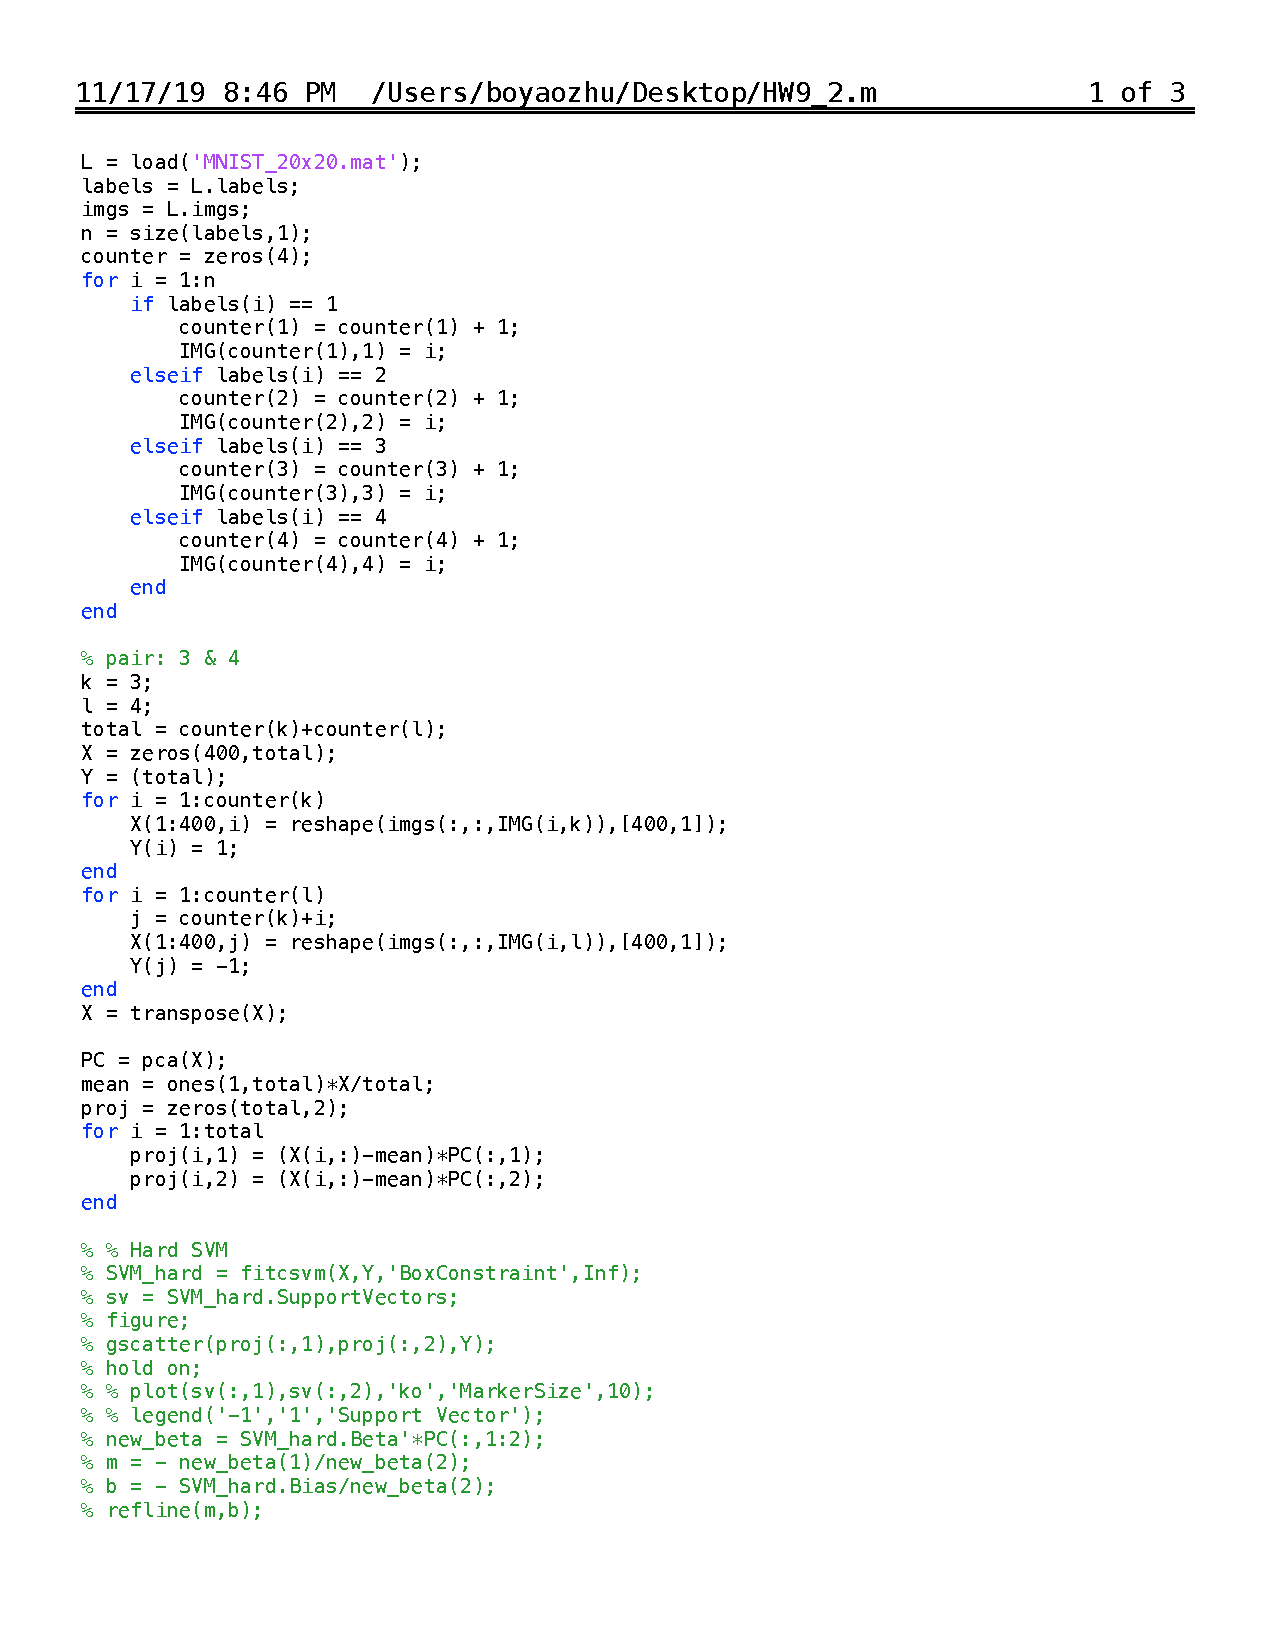
\includepdf[page={-}]{2.pdf}
















\end{document}